% Schema
\section{Userspace}
	\begin{frame}
		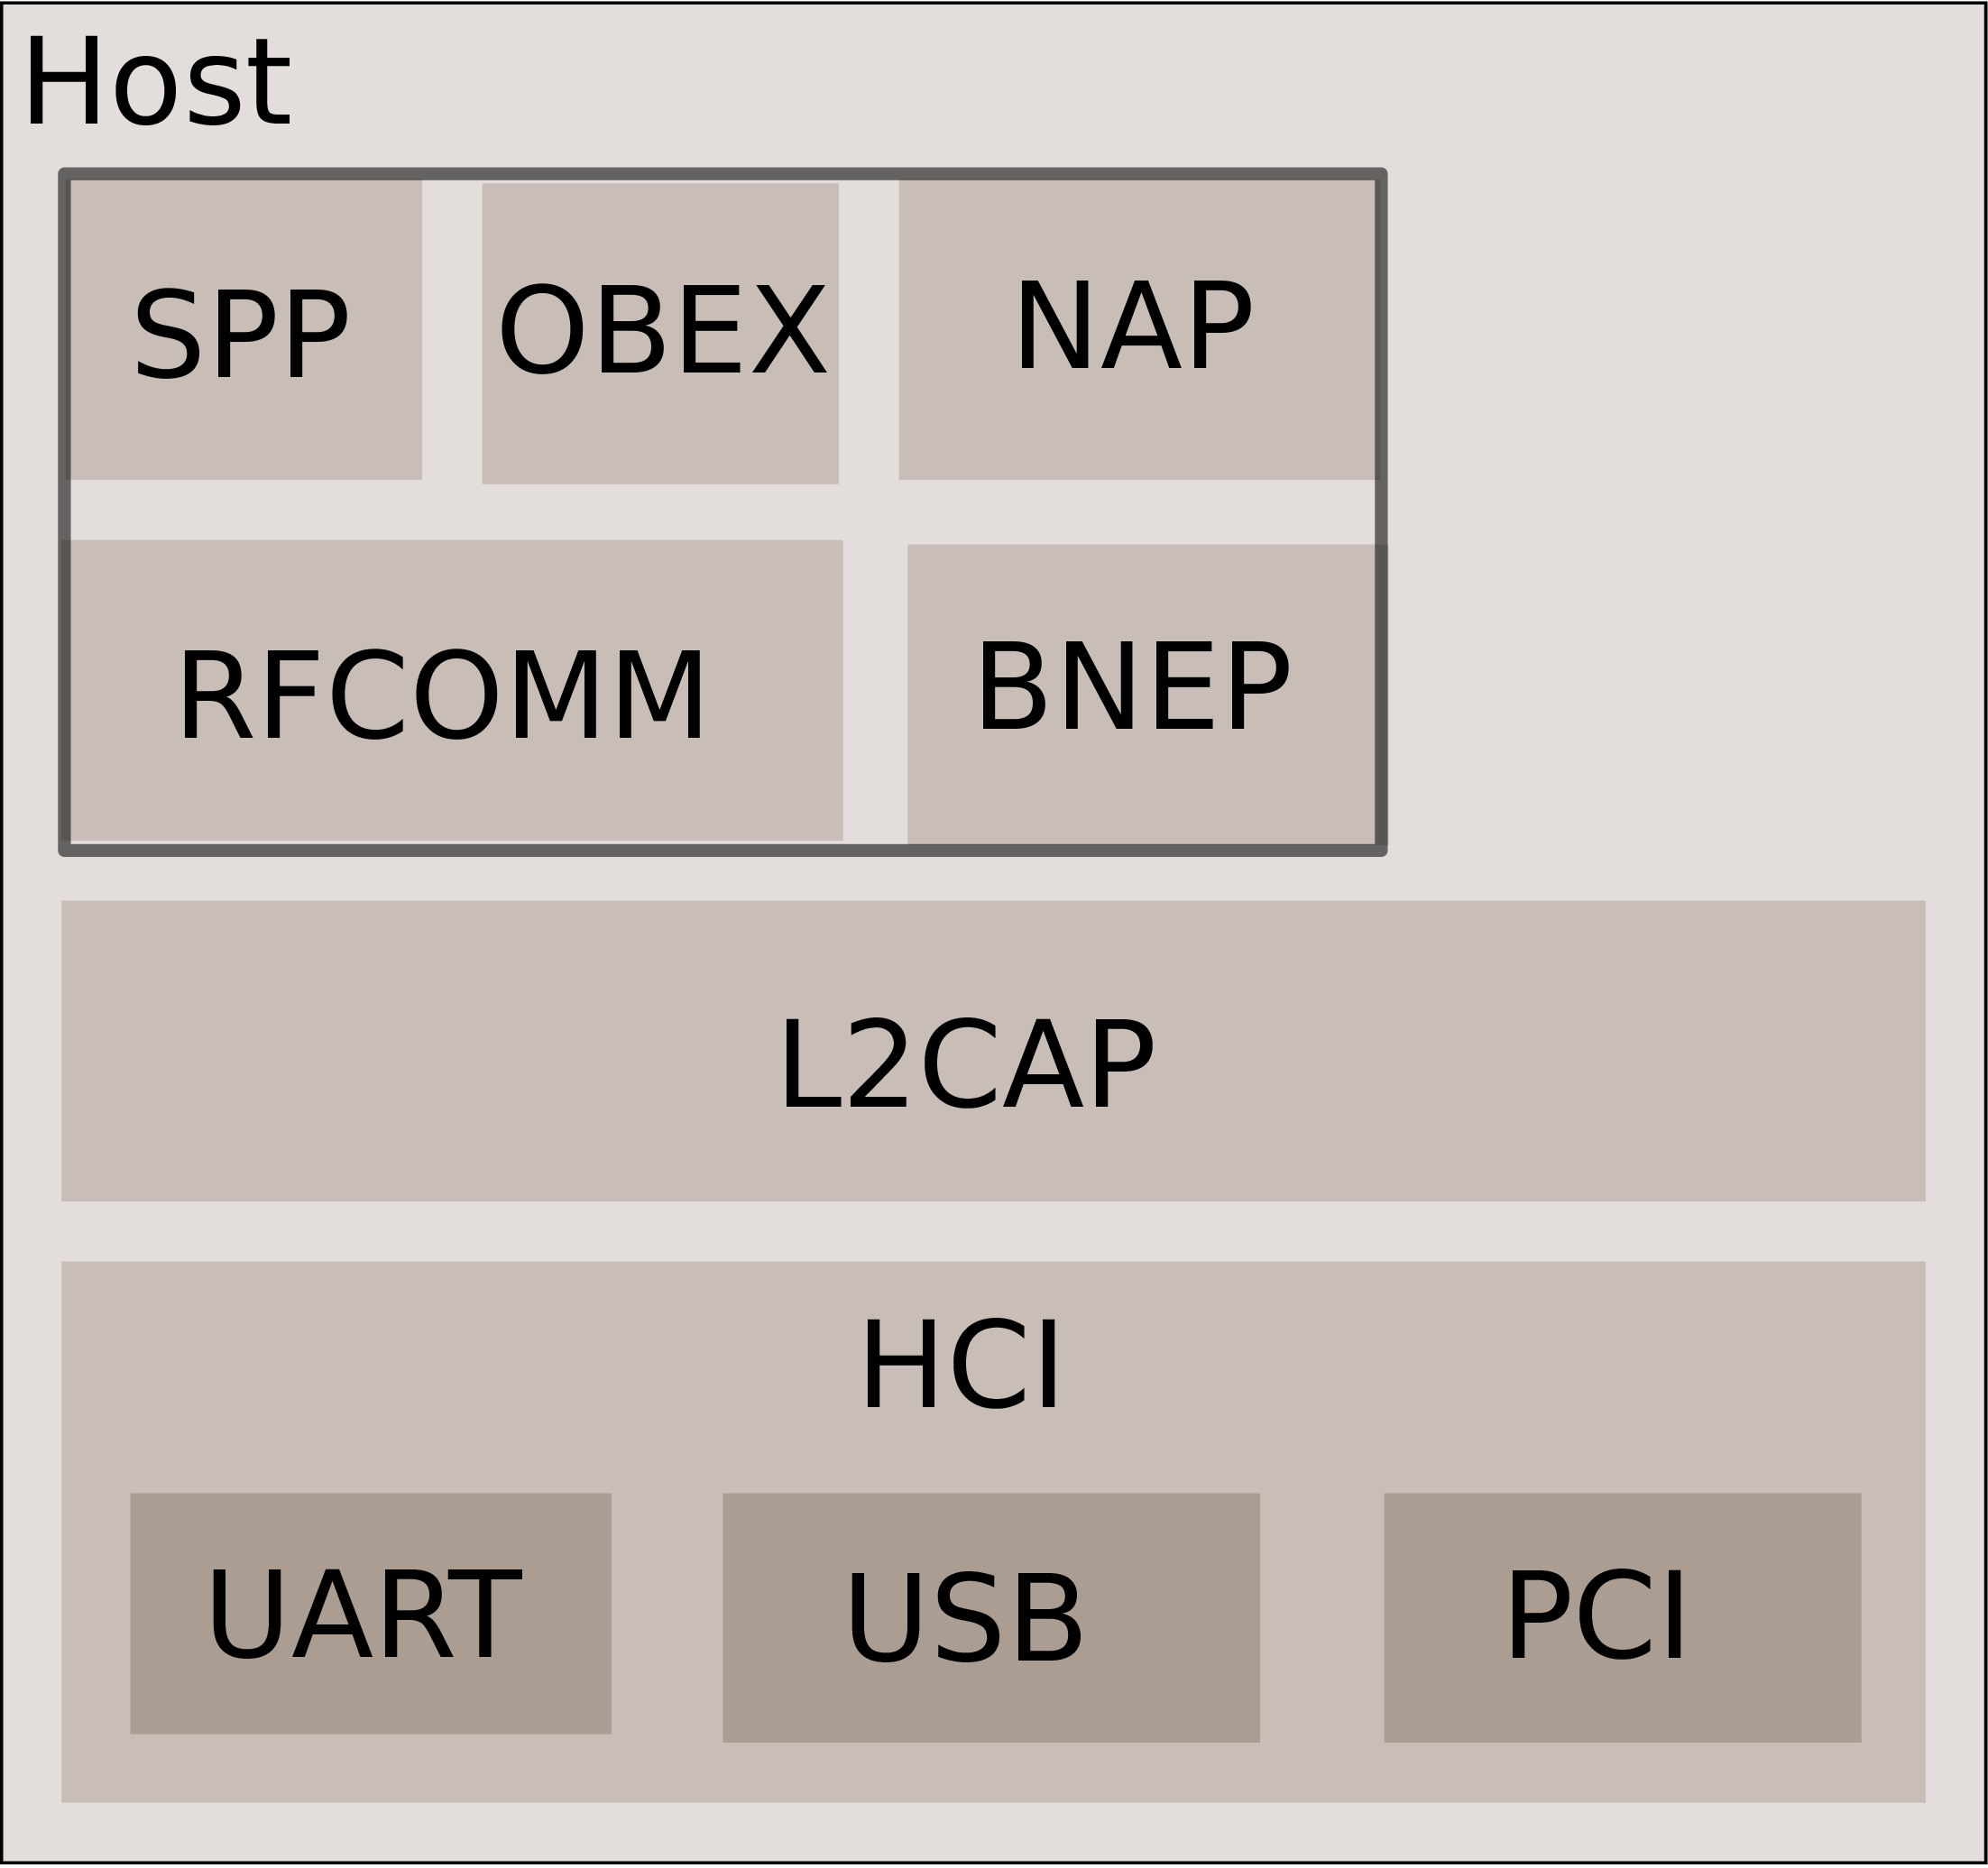
\includegraphics[height=5cm]{img/arch_log_all.png}
		\caption{kernel + userspace}
	\end{frame}
	\begin{frame}
		\center{\huge{Système d'init}}
		\begin{itemize}
			\item Premier processus lancé
			\item Lance les autres processus
			\item Influe sur le temps de boot
		\end{itemize}
		\begin{block}{SysV init}
			\begin{itemize}
				\item Scripts
				\item Peu de parallélisation
			\end{itemize}
		\end{block}
		\begin{block}{Systemd}
			\begin{itemize}
				\item Fichiers de configuration
				\item Parallélisation et dépendances
				\item Plus complexe
			\end{itemize}
		\end{block}
	\end{frame}

\subsection{libC}
% choix de la libC
\subsection{Outils}
% choix des libs
\subsection{Librairies}
% choix des outils ( busybox, vrai outils )
